\documentclass[12 pt]{article}        	
\usepackage{amsfonts, amssymb, amsmath, graphicx}

\oddsidemargin=-0.5cm

\setlength{\textwidth}{6.5in}         	
\addtolength{\voffset}{-20pt}        	
\addtolength{\headsep}{25pt}

\pagestyle{myheadings}

\markright{Juani Elosegui \hfill \today \hfill}

\begin{document}

\subsection*{Ejercicio 2}
    \subsubsection*{(a)}
        El invariante correcto es el siguiente:
        \\
        $\mathcal{I}_{2}: (1 \leq i \leq N+1) \wedge (res = \sum^{i-1}_{j=0}j^{2})$
        \begin{itemize}
            \item Notar que $i$ terminará valiendo uno más que N, por eso digo que va hasta N+1.
            \item El índice de la sumatoria es $j$, que funciona de manera análoga con el índice propuesto $i$. Cambiamos de nombre de índice para que no haya confusiones.
        \end{itemize}
    \subsubsection*{(b)}
        Precondición $P_{c}: (N>0) \wedge (i=1) \wedge (res=0)$
        \begin{itemize}
            \item Hay que incluir también la precondición de la función en sí. Todo lo que sepas antes del ciclo, hay que incluirlo.
        \end{itemize}
        Postcondición $Q_{c}: (i=N+1) \wedge (res=\sum^{N}_{i=1}i^{2})$
        \begin{itemize}
            \item $i$ terminará valiendo N+1 porque hay que contar la iteración en la cual la guarda se vuelve falsa.
            \item En la postcondición, se debe explicar el proceso del loop en términos de la guarda (en este caso, N).
        \end{itemize}
    \subsubsection*{(c)}
        $i=3, N=3, res=5$:
        \begin{itemize}
            \item Cumple el invariante, porque $(1 \leq 3 \leq 3+1) \wedge (5 = \sum^{3-1}_{j=0}j^{2})$
            \item Cumple la guarda del ciclo, porque $3 \leq 3$.
        \end{itemize}
    \subsubsection*{(d)}
        \begin{itemize}
            \item $(i=3) \wedge (N=3) \wedge (res=5)$
            \item $(i=3) \wedge (N=3) \wedge (res=5+3\cdot3)$
            \item $(i=4) \wedge (N=3) \wedge (res = 14)$
        \end{itemize}
    \subsubsection*{(e)}
        \[P_{c} \Rightarrow \mathcal{I}\]
        \[(N>0) \wedge (i=1) \wedge (res=0) \Rightarrow (1 \leq i \leq N+1) \wedge (res=\sum^{i-1}_{j=0}j^{2})\]
        Como $N$ es mayor que cero, se puede asumir que $N \geq 1$. Por lo que podemos cambiar eso.
        \[(N \geq 1) \wedge (i=1) \wedge (res=0) \Rightarrow (1 \leq i \leq N+1) \wedge (res=\sum^{i-1}_{j=0}j^{2})\]
        Podemos ver que se cumple el primer término de $\mathcal{I}$, porque $1 \leq 1 \leq 1+1$ es verdadero.
        \\
        También se cumple el segundo término, porque $0 = \sum^{1-1}_{j=0}j^{2}$. Se cumple ya que si el límite de la sumatoria es cero, la sumatoria en sí da cero, por lo que $0=0$ es verdadero.
    \subsubsection*{(f)}
        \[\neg B \wedge \mathcal{I} \Rightarrow Q_{c}\]
        \[(i > N) \wedge \left((1 \leq i \leq N+1) \wedge (res=\sum^{i-1}_{j=0}j^{2})\right) \Rightarrow (i=N+1)\]

        \begin{itemize}
            \item $(i=N+1)$ vale, porque por $\mathcal{I}$ teníamos que $(1 \leq i \leq N+1)$.
        \end{itemize}

\subsection*{Ejercicio 3}
    \subsubsection*{(a)}
        \begin{center}
            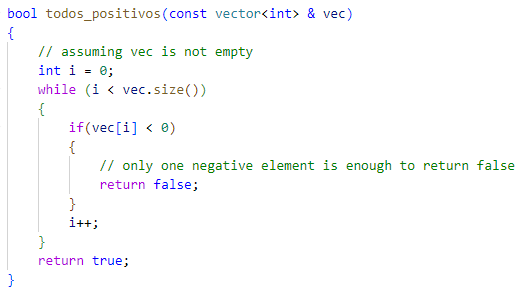
\includegraphics[width=0.55 \linewidth]{g3_codes/p3.1.PNG}
        \end{center}
        \begin{itemize}
            \item $P_{c}: (|vec| \geq 1) \wedge (i = 0)$
            \item $Q_{c}$: \textit{if} $\left(\sum^{|vec|-1}_{i=0}\beta (esPositivo(vec[i])) = |vec|-1\right)$ \textit{then} res = True \textit{else} res = False \textit{fi} $\wedge (i = |vec|)$

            esPositivo (i:int) $\equiv i > 0$

            \item $\mathcal{I}: (0 \leq i \leq |vec|) \wedge \left(res = True \Leftrightarrow \sum^{i-1}_{j=0} \beta (esPositivo(vec[j])) = |vec|-1 \right)$
        \end{itemize}

    \subsubsection*{(b)}
        \begin{center}
            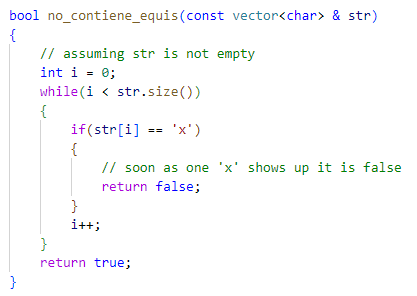
\includegraphics[width=0.35 \linewidth]{g3_codes/p3.2.PNG}
        \end{center}
        \begin{itemize}
            \item $P_{c}: (|str| \geq 1) \wedge (i=0)$
            \item $Q_{c}: $\textit{if} $(1 \leq \sum^{|str|-1}_{i=0}\beta($esX (str[i]$)) \leq |str|-1)$ \textit{then} (res = False) \textit{else} (res = True) \textit{fi} $\wedge (i = |str|)$

            esX (c:char) $\equiv c = 'x'$

            Si la cantidad de ocurrencias de `x' está entre 1 y el tamaño de str, quiere decir que sí apareció una `x', por lo que es falso.
        \end{itemize}

\subsection*{Ejercicio 4}
    \begin{itemize}
        \item $P_{c}: (i \geq 0) \wedge (n \geq i) \wedge (res \geq 1)$
        \item $Q_{c}: (res = \prod^{N}_{i=0}i) \wedge (i = n + 1)$
        \item $\mathcal{I}: (0 \leq i \leq n+1) \wedge (res = \prod^{i-1}_{j=0}j)$
    \end{itemize}

\subsection*{Ejercicio 5}
    \subsubsection*{(a)}
        \begin{itemize}
            \item $P_{c}: (N > 0) \wedge (i = 1) \wedge (res = 2)$
            \item $Q_{c}: (i = N) \wedge (res = \sum^{N - 1}_{i = 1}\beta(N$ mod $i = 0))$
        \end{itemize}
    \subsubsection*{(b)}
        El invariante correcto es $\mathcal{I}_{3}$.
    \subsubsection*{(c)}
        \begin{itemize}
            \item $i = 1, N = 4$
            \item Cumple que $1 \leq 2 < 4$ y que $2 = 2 * 1$
        \end{itemize}
    \subsubsection*{(d)}

\subsection*{Ejercicio 6}
    \subsubsection*{(a)}
        \begin{center}
            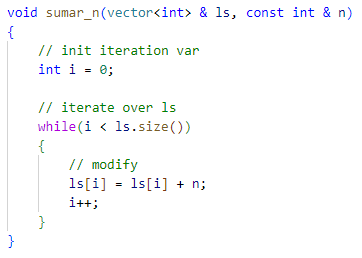
\includegraphics[width=0.4 \linewidth]{g3_codes/p6.1.PNG}
        \end{center}
        \begin{itemize}
            \item $P_{c}: (i=0)$
            \\
            Sólo la variable de iteración. No es necesario agregar nada más, ni siquiera alguna precondición del programa.
            \item $Q_{c}: (|ls_{0}| = |ls|) \wedge (i = |ls|) \wedge (\forall i$:int$)(0 \leq i \leq |ls| \Rightarrow ls[i] = ls_{0}[i] + n)$
            \\
            El tamaño del vector inicial se mantiene luego de modificar sus elementos. $i$ terminará valiendo $|ls|$ porque se debe incumplir la guarda en algún momento. Todos los elementos de $ls$ serán los elementos de $ls_{0}$ sumado $n$.
            \item $\mathcal{I}: (0 \leq i \leq |ls|) \wedge (\forall j$:int$)(0 \leq j < i \Rightarrow ls[j] = ls_{0}[j] + n)$
            \\
            $i$ parte desde cero por la precondición y terminará valiendo lo que el tamaño de $ls$. Todos los valores de $j$ entre cero e $i$ irán modificando los valores de $ls_{0}$. Uso $j$ para diferenciarlo de $i$.
        \end{itemize}
    \subsubsection*{(b)}
        \begin{center}
            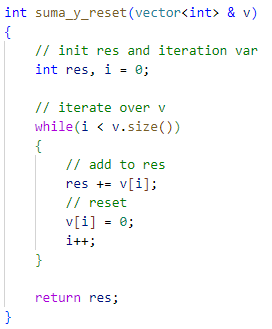
\includegraphics[width=0.4 \linewidth]{g3_codes/p6.2.PNG}
        \end{center}
        \begin{itemize}
            \item $P_{c}: (i = 0) \wedge (res = 0)$
            \\
                Por la declaración de estas variables en cero.
            \item $Q_{c}: \left(res = \sum^{|v_{0}|-1}_{i=0}v_{0}[i]\right) \wedge (i = |v_{0}| = |v|) \wedge (\forall i$:int$)(0 \leq i \leq |v| \Rightarrow v[i] = 0)$
            \\
                $res$ es la sumatoria de todos los valores en $v_{0}$. $i$ va a terminar siendo igual al tamaño de $v_{0}$, y, como no vamos a cambiar el tamaño del vector, se mantiene que $|v_{0}| = |v|$. Como reseteamos todos los valores, tenemos que todos los valores del vector modificado, $v$, serán cero.
            \item $\mathcal{I}: \left(res = \sum^{i-1}_{j=0}v_{0}[j]\right) \wedge (\forall j$:int$)(0 \leq j < i \Rightarrow v[j] = 0) \wedge (0 \leq i \leq |v|)$
            \\
                $res$ es la sumatoria desde $j$ hasta $i-1$. Se puede decir que $j$ ``va por atrás de $i$'' modificando las cosas. Importante aclarar el rango de valores de $i$.
        \end{itemize}

\subsection*{Ejercicio 7}
    \begin{center}
        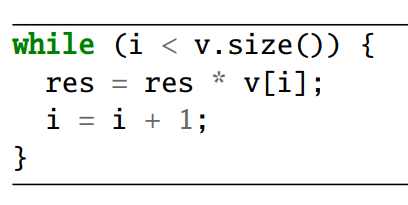
\includegraphics[width=0.35 \linewidth]{g3_consignas/p7.PNG}
    \end{center}
    \begin{itemize}
        \item $P_{c}: (|v| \geq 1) \wedge (res \neq 0)$
        \\
            Si $res$ fuera cero, no tendría sentido que multipliquemos todo por cero. Además, $v$ debería tener al menos un elemento para acceder, para que no se indefina en la primera línea de la iteración.
        \item $Q_{c}: \left(res = \prod^{|v|-1}_{i=0}v[i]\right) \wedge (i = |v|)$
        \\
            $res$ será la productoria de todos los elementos de $v$. $i$ terminará valiendo $|v|$ porque necesitamos que el iterador termine en algún momento.
        \item $\mathcal{I}: \left(res = \prod^{i-1}_{j=0}v[j]\right) \wedge (0 \leq i \leq |v|)$
            $res$ es la productoria de todos los índices $j$ que van ``por detrás'' de $i$. El rango de $i$ está aclarado.
    \end{itemize}

\subsection*{Ejercicio 8}
    \begin{center}
        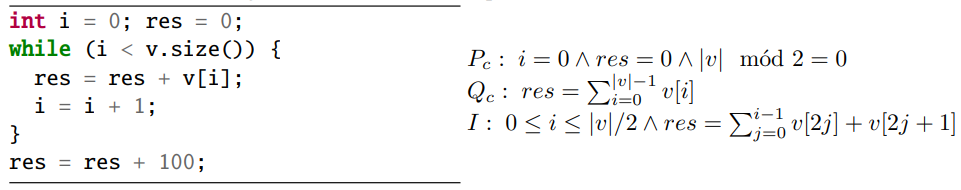
\includegraphics[width=0.9\linewidth]{g3_consignas/p8.PNG}
    \end{center}
    \subsubsection*{(a)}
        El invariante no respeta al código, porque $i$ termina adquiriendo el valor de $|v|$ para la última iteración (esto es $0 \leq i \leq |v|$). Además, la suma de los elementos de $v$ a $res$ son comunes, no es que esté mal la sumatoria en sí (porque llegaríamos al mismo resultado de $res)$, pero no es precisamente lo que hace el iterador.
    \subsubsection*{(b)}
        Me piden:
        \begin{itemize}
            \item Vector de tamaño par.
            \item Inicializar las variables de iteración y la respuesta en 0.
            \item Cuando termine el ciclo, $res$ será la sumatoria de todos sus elementos.
            \item La iteración llegará a la mitad del vector, y se sumarán a $res$ todos los elementos de a ``parejas''.
        \end{itemize}
        \begin{center}
            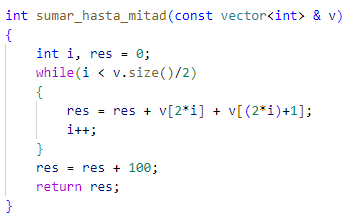
\includegraphics[width=0.5 \linewidth]{g3_codes/p8.1.PNG}
        \end{center}
    \subsubsection*{(c)}
        \begin{center}
            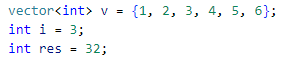
\includegraphics[width=0.5 \linewidth]{g3_codes/p8.2.PNG}
        \end{center}
        \begin{itemize}
            \item Cumplen el invariante porque: $0 \leq 3 \leq 6/2 = 3$ y 
            
            $32 = \sum^{3-1 = 2}_{j = 0}v[2j]+v[2j+1] \Rightarrow $ 
            
            $32 = (0+v[0]+v[1])+(3+v[2]+v[3])+(10+v[3]+v[4]) \Rightarrow$ 
            
            $32 = (0+1+2)+(3+3+4)+(10+4+5) \Rightarrow $

            $32 = 3+10+19 \Rightarrow $

            $32 = 32$
        \end{itemize}
    \subsubsection*{(e)}
        \begin{itemize}
            \item Satisface el invariante, porque $0 \leq 3 \leq 3$. Como dije arriba.
            \item No satisface la guarda, porque $3 < 6/2$ es falso.
            \item Satisface la postcondición $P_{c}$, porque $\ldots$ ``no entendí el código, porque según lo que entendí, suma todos los números menos el último. ¿Estará bien escrito lo de $res$ en el código? Parece que estoy acumulando los resultados de cada iteración anterior. Yo sé que debería ser la suma de todos los elementos del vector''.
        \end{itemize}
    \subsubsection*{(f)}
        Quiero demostrar que $\neg B \wedge \mathcal{I} \Rightarrow Q_{c}$
        
        $\equiv \left(i \geq |v|/2\right) \wedge \left(0 \leq i \leq |v|/2 \wedge res = \sum^{i-1}_{j=0}v[2j]+v[2j+1]\right) \Rightarrow \left(res = \sum^{|v|-1}_{i=0}v[i]\right)$

        \begin{itemize}
            \item La postcondición vale, porque si tomamos que $i \geq |v|/2 \wedge i \leq |v|/2$ tenemos que $|v|/2 = i \Rightarrow |v| = 2i$. Si reemplazamos $|v|$ en el límite de la sumatoria esta se anulará porque quedaría $res = \sum^{2i = 0}_{i=0}v[i] = 0$.
        \end{itemize}
        
\subsection*{Ejercicio 9}
     \begin{center}
         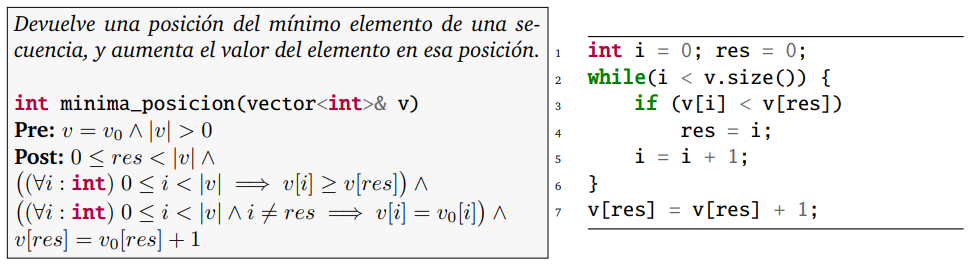
\includegraphics[width=0.8 \linewidth]{g3_consignas/p9.PNG}
     \end{center}
     \subsubsection*{(a)}
        \begin{itemize}
            \item $P_{c}: (v = v_{0}) \wedge (|v| > 0) \wedge (i = 0) \wedge (res = 0)$
            \\
                Incluimos las cosas de la precondición de la función, y las declaraciones de variables.
            \item $Q_{c}: (0 \leq res < |v|) \wedge (\forall i$:int$)(0 \leq i < |v| \Rightarrow v[i] \geq v[res]) \wedge $
            
            $(\forall i$:int$)(0 \leq i < |v| \wedge i \neq res \Rightarrow v[i] = v_{0}[i]) \wedge (i = |v|)$
            \\
                Copié las pre y postcondiciones de la función, menos la línea en la que se incrementa el mínimo elemento. Además, $i$ terminará adquiriendo el valor de $|v|$ porque se deja de cumplir la guarda.
            \item $\mathcal{I}: (0 \leq i \leq |v|) \wedge (0 \leq res < |v|) \wedge (\forall j$:int$)(0 \leq j < i \Rightarrow v[res] \leq v[j])$
            \\
                Defino los rangos de $i$ y de $res$. Notar que $res$ no puede ser $|v|$. Explico que todo elemento en el índice $j$ será mayor al elemento en el índice $res$. 
        \end{itemize}
    \subsubsection*{(b)}
        Quiero probar que $\mathcal{I} \wedge \neg B \Rightarrow Q_{c}$.
        \\
        $\left((0 \leq i \leq |v|) \wedge (0 \leq res < |v|) \wedge (\forall j:int)(0 \leq j < i \Rightarrow v[res] \leq v[j])\right)$
        \\
        $\wedge \left(i \geq |v|\right)$
        \\
        $\Rightarrow (0 \leq res < |v|) \wedge (\forall i$:int$)(0 \leq i < |v| \Rightarrow v[i] \geq v[res]) \wedge $
        \\
        $(\forall i$:int$)(0 \leq i < |v| \wedge i \neq res \Rightarrow v[i] = v_{0}[i]) \wedge (i = |v|)$
        \begin{itemize}
            \item Por $(i \leq |v|) \wedge (i \geq |v|) \Rightarrow (i = |v|)$ del invariante y la guarda negada, tenemos que es válido que $(i = |v|)$ vale en la postcondición.
        \end{itemize}

\subsection*{Ejercicio 10}
    \begin{center}
        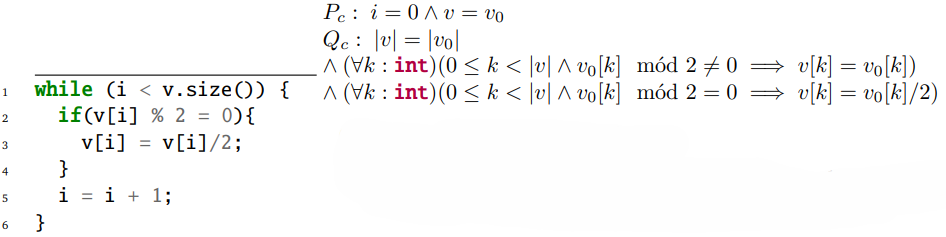
\includegraphics[width=0.75 \linewidth]{g3_consignas/p10.PNG}
    \end{center}
    \subsubsection*{(a)}
        $\mathcal{I}: (0 \leq i \leq |v|) \wedge (\forall j$:int$)(0 \leq j < i \wedge v_{0}[j]$ mod $2 = 0 \Rightarrow v[j] = v_{0}[j]/2)$
        \\
        $i$ va a llegar al valor de $|v|$, y todos los elementos en $v[j]$ pares se van a dividir por dos.\textit{ ¿Es necesario aclarar qué pasa si el elemento es impar?}
    \subsubsection*{(b)}
        Tenemos $i = 0$ y que $v_{0} = \{4, 3, 1, 8\}$ con $|v_{0}| = 4$. Preservará el invariante porque $0 \leq 0 \leq 4$. La ejecución terminará con $|v_{0}| = 4$, $v = \{2, 3, 1, 8\}$ y con $i = 1$.
    \subsubsection*{(c)}
        La función variante es $f_{v}: |v| - i$. Esta función es estrictamente decreciente en función de $i$. Si esta función llega a cero, quiere decir que $f_{v} = 0 \Rightarrow |v|-i = 0$. Esto se cumple si $i = |v|$.
        \\
        La guarda $B$ se hace falsa cuando $i \geq |v|$, y cuando $i = |v|$ (que es cuando la función variante se hace cero) se cumple la terminación del ciclo.

\subsection*{Ejercicio 11}

\subsection*{Ejercicio 12}
    \subsubsection*{(a)}
        \begin{center}
            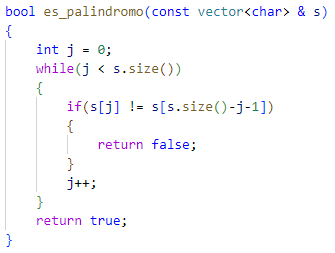
\includegraphics[width=0.5 \linewidth]{g3_codes/p12.1.PNG}
        \end{center}
    \subsubsection*{(b)}
        \begin{center}
            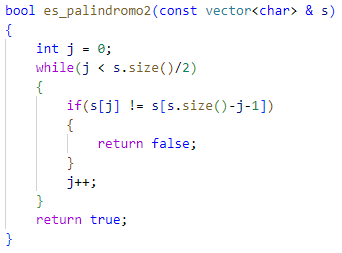
\includegraphics[width=0.5 \linewidth]{g3_codes/p12.2.PNG}
        \end{center}

\subsection*{Ejercicio 13}
    \subsubsection*{(a)}
        \begin{center}
            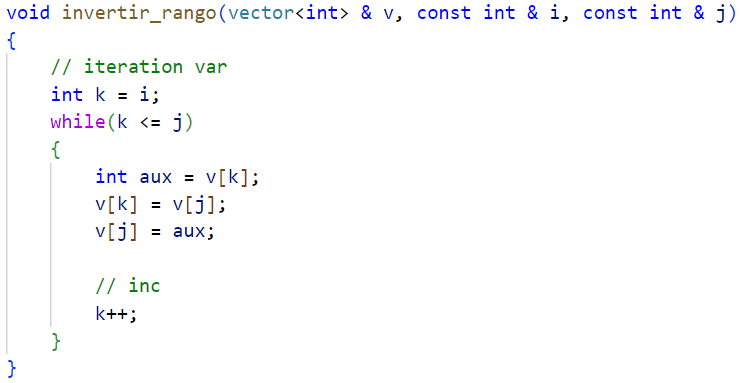
\includegraphics[width=0.65 \linewidth]{g3_codes/p13.1.PNG}
        \end{center}
    \subsubsection*{(b)}
        \begin{itemize}
            \item $P_{c}: \left(0 \leq i < |v|\right) \wedge \left(0 \leq j < |v|\right) \wedge (i \leq j) \wedge (k = i)$
            \\
            $i$ y $j$ están en el rango de $v$. $i$ es menor o igual que $j$. Para iterar, $k$ es igual a $i$.
            \item $Q_{c}: (\forall k$:int$)\left(0 \leq k < \min(i, j) \vee \max(i, j) < k < |v| \Rightarrow (v[k] = v_{0}[k])\right)$
            
            $\wedge \left(\min(i, j) \leq k \leq \max(i, j) \Rightarrow v[k] = v_{0}[\min(i, j)+\max(i, j)-k]\right)$

            $\wedge (k = j+1) \wedge (|v|=|v_{0}|)$
            \\
            Además de la postcondición del problema, también aclaré que $k = j+1$ porque se tiene que negar la guarda, y se mantiene el tamaño del vector.
            \item $\mathcal{I}: (i \leq k \leq j+1) \wedge (\forall k$:int$)\left(0 \leq k < \min(i, j) \vee \max(i, j) < k < |v| \Rightarrow (v[k] = v_{0}[k])\right) $
            
            $\wedge \left(\min(i, j) \leq k \leq \max(i, j) \Rightarrow v[k] = v_{0}[\min(i, j)+\max(i, j)-k]\right)$
        \end{itemize}
        
\subsection*{Ejercicio 14}
    \begin{center}
        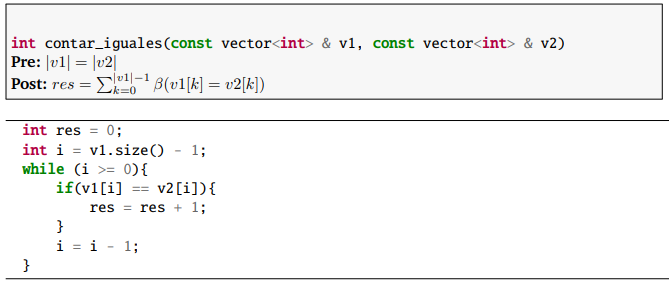
\includegraphics[width=0.75 \linewidth]{g3_consignas/p14.PNG}
    \end{center}
    \subsubsection*{(a)}
        \begin{itemize}
            \item $P_{c}: (|v_{1}| = |v_{2}|) \wedge (res = 0) \wedge (i = |v_{1}|-1)$
            \\
            Agrego la precondición de la función y la declaración de las variables antes de que empiece el ciclo.
            \item $Q_{c}: \left(res = \sum^{|v_{1}|-1}_{i = 0}\beta(v_{1}[k] = v_{2}[k])\right) \wedge (i = -1)$
            \\
            $res$ será la sumatoria de todos los elementos que sean iguales en los dos vectores desde $i$ hasta el final de un vector, ya que sabemos que los dos tienen el mismo tamaño. 
            \item $\mathcal{I}: (-1 \leq i \leq |v_{1}|-1) \wedge \left(res = \sum^{i+1}_{j=0}\beta(v_{1}[j] = v_{2}[j])\right)$
            \\
            $i$ va desde $|v_{1}|-1$ hasta $-1$ porque se tiene que negar la guarda.
        \end{itemize}
    \subsubsection*{(b)}
        \begin{center}
            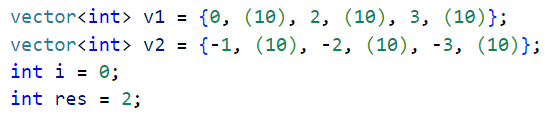
\includegraphics[width=0.65 \linewidth]{g3_codes/p14.1.PNG}
        \end{center}
        \begin{itemize}
            \item Cumple el invariante, porque $-1 \leq 0 \leq 6 - 1$ y $2 = (0)+(1)+(0)+(1)+(0)$.
            \item Se cumple la guarda del ciclo, porque $0 \geq 0$.
        \end{itemize}
    \subsubsection*{(c)}
        En la última iteración sabíamos que $i = 0, res = 2$. Como se cumple la condición del \textit{if}, $res = 2+1$. Finalmente, $i = -1$.
    \subsubsection*{(d)}
        $res = 3, i = -1$. 
        \begin{itemize}
            \item Esto cumple el invariante porque $3 = (1)+(0)+(1)+(0)+(1)+(0)$ y $-1 \leq -1 \leq 6$.
            \item No cumple con la guarda del ciclo porque $-1 \geq 0$ es falso.
            \item También cumple con la postcondición porque $i = -1$ y $3 = (1)+(0)+(1)+(0)+(1)+(0)$.
        \end{itemize}

\subsection*{Ejercicio 15}
    \subsubsection*{(a)}
        \begin{center}
            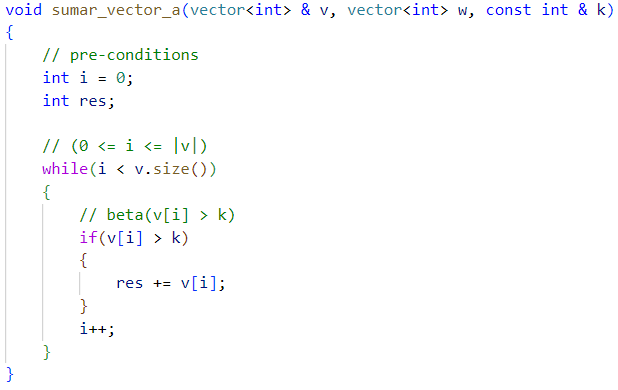
\includegraphics[width=0.65 \linewidth]{g3_codes/p15.1.PNG}
        \end{center}
    \subsubsection*{(b)}
        \begin{center}
            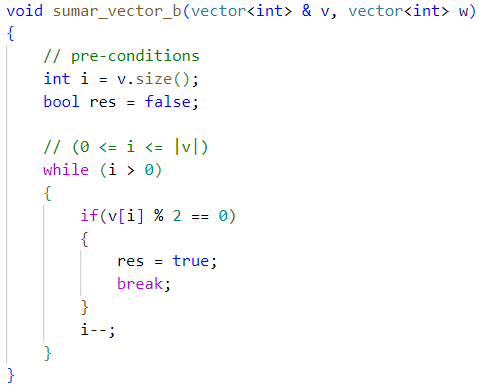
\includegraphics[width=0.5 \linewidth]{g3_codes/p15.2.PNG}
        \end{center}
    \subsubsection*{(c)}
        \begin{center}
            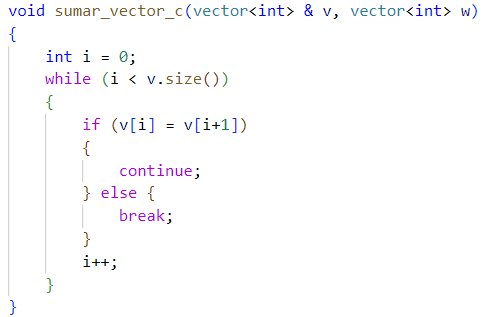
\includegraphics[width=0.5 \linewidth]{g3_codes/p15.3.PNG}
        \end{center}
    \subsubsection*{(d)}
        \begin{center}
            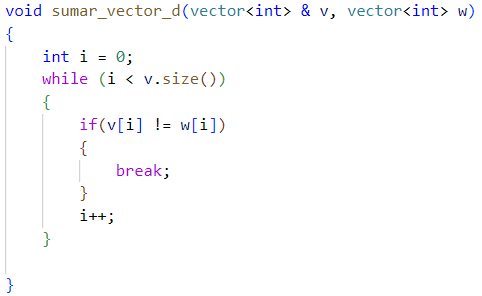
\includegraphics[width=0.5 \linewidth]{g3_codes/p15.4.PNG}
        \end{center}

\end{document}